%template for producing IEEE-format articles using LaTeX.
%written by Matthew Ward, CS Department, Worcester Polytechnic Institute.
%use at your own risk.  Complaints to /dev/null.
%make two column with no page numbering, default is 10 point



\documentclass[twocolumn]{article}
\usepackage[pdftex]{graphicx}
\pagestyle{empty}
\usepackage[utf8]{inputenc} 


\renewcommand*\familydefault{\sfdefault} 
\usepackage[scaled]{helvet} %para usar helvetica
\renewcommand\familydefault{\sfdefault} 
\usepackage[T1]{fontenc}

%set dimensions of columns, gap between columns, and space between paragraphs
\setlength{\textheight}{8.75in}
\setlength{\columnsep}{2.0pc}
\setlength{\textwidth}{6.8in}
%\setlength{\footheight}{0.0in}
\setlength{\topmargin}{0.25in}
\setlength{\headheight}{0.0in}
\setlength{\headsep}{0.0in}
\setlength{\oddsidemargin}{-.19in}
\setlength{\parindent}{1pc}

%I copied stuff out of art10.sty and modified them to conform to IEEE format

\makeatletter
%as Latex considers descenders in its calculation of interline spacing,
%to get 12 point spacing for normalsize text, must set it to 10 points
\def\@normalsize{\@setsize\normalsize{12pt}\xpt\@xpt
\abovedisplayskip 10pt plus2pt minus5pt\belowdisplayskip \abovedisplayskip
\abovedisplayshortskip \z@ plus3pt\belowdisplayshortskip 6pt plus3pt
minus3pt\let\@listi\@listI} 

%need an 11 pt font size for subsection and abstract headings
\def\subsize{\@setsize\subsize{12pt}\xipt\@xipt}

%make section titles bold and 12 point, 2 blank lines before, 1 after
\def\section{\@startsection {section}{1}{\z@}{24pt plus 2pt minus 2pt}
{12pt plus 2pt minus 2pt}{\large\bf}}

%make subsection titles bold and 11 point, 1 blank line before, 1 after
\def\subsection{\@startsection {subsection}{2}{\z@}{12pt plus 2pt minus 2pt}
{12pt plus 2pt minus 2pt}{\subsize\bf}}
\makeatother

\usepackage{graphicx}  
\newcommand{\imgdir}{doc-img} 
\graphicspath{{\imgdir/}} 
\usepackage{amsmath}


\begin{document}


%don't want date printed
\date{}

%make title bold and 14 pt font (Latex default is non-bold, 16 pt)
\title{\Large\bf Análisis de liberación de catecolaminas en células cromafinas de ratón mediante Amperometría}

%for single author (just remove % characters)
\author{J. Palma-Espinosa \\
  Laboratorio de Neurociencia Computacional - CNScLAB \\
  Universidad Valparaíso. Valparaíso, Chile \\
  javier.palma@cinv.cl}
 
%for two authors (this is what is printed)
%\author{\begin{tabular}[t]{c@{\extracolsep{8em}}c}
%  I. M. Author	& M. Y. Coauthor \\
% \\
%  My Department & Coauthor Department \\
%  My Institute & Coauthor Institute \\
%  City, ST~~zipcode	& City, ST~~zipcode
%\end{tabular}}

\maketitle

%I don't know why I have to reset thispagesyle, but otherwise get page numbers
\thispagestyle{empty}

\subsection*{\centering Abstract}
%IEEE allows italicized abstract
{\em
In the past 10 years, the industry has strongly benefit from the wireless sensor network technology.  However, the harsh environment in which this networks are deployed, makes urgent to develop empirical and computational models that predict the network performance in such hostile environment.
One particular harsh environment is the minning industry, in which the physical characteristics of the tunnel and rooms make this modeling even harder.
A review of those models is presented, together with suggestions of possible continuation of the presented works\\
{\bf Keywords: WSN, Channel modeling, minning industry, Zigbee, IEEE 802.15.4}
}


\section{Introducción}
En un organismo pluricelular, las células deben interpretar las numerosas señales que reciben desde otras células\cite{alberts2006introduccion}. Estas señales, generan respuestas químicas que permiten coordinar no sólo su propio comportamiento, sino también generar respuestas a una escala superior, que permita la supervivencia de dicho organismo \cite{jarukanont2015vesicle}.
Esta cadena de interpretación y generación de señales suele realizarse por vías químicas, mediante la exocitosis regulada de moléculas bioquímicas\cite{evanko2005primer, aspinwall1999comparison}, tales como catecolaminas, serotonina y péptidos \cite{mosharov2005analysis}, que desencadenarán la respuesta deseada en la célula blanco, en particular.
Durante este proceso, la célula que porta el mensaje, libera moléculas mensajeras  al medio extracelular, en un proceso llamado exocitosis\cite{gonzalez2010association}, el cual se produce cuando vesículas portadoras de las moléculas señalizadoras, generan un poro de fusión entre las membranas de la vesícula y la célula\cite{amatore2009quantitative,oleinick2013vesicular}, generando un flujo de tales moléculas hacia el medio extracelular, o espacio sináptico en el caso de neuronas.
Actualmente, se conocen tres modelos por los cuales se produce la exocitosis de moléculas mensajeras: Colapso-fusión completa, kiss and run y exocitosis compuesta\cite{wu2014exocytosis}.  
El modelo de exocitosis de fusión completa propone que la vesícula transportadora comienza a fusionarse con la membrana celular, generando un espacio , de forma tal que esta fusión provoca una liberación de las moléculas señalizadoras hacia el medio extracelular
Amperometry provides valuable information on the fine kinetics of transmitter release during vesicular exocytosis and hence has had a great influence on the current view of vesicle exocytosis and the existence of fusion pores[friedrich2010spike]


\section{Materiales y Métodos}
\subsection{Cultivo celular y preparación}
blabalbal cromafina de raton

\subsection{Registro}



\subsection{Análisis de datos}

\begin{table*}
\label{tab:ieee}
  \centering
	\begin{tabular}{ | c | c | c | c | }
	  \hline
	  Characteristic & Europe & USA & Worldwide \\
	  \hline
	  Frequency Assignment & 868 to 868.6 MHz & 902 to 928 MHz & 2.4 to 2.4835 GHz\\
	  \hline
	  Number of Channels & 1 & 10 & 16\\
	  \hline
	  Channel Bandwidth & 600 kHz & 2 MHz & 5 MHz\\
	  \hline
	  Data Rate & 20 kbps & 20 kbps & 250 kbps\\
	  \hline
	  Modulation & BPSK & BPSK & O-QPSK\\
	  \hline
	\end{tabular}
	\caption{Definitions of the PHY layer for IEEE 802.15.4}
\end{table*}

\begin{figure*}[h!]
\centering
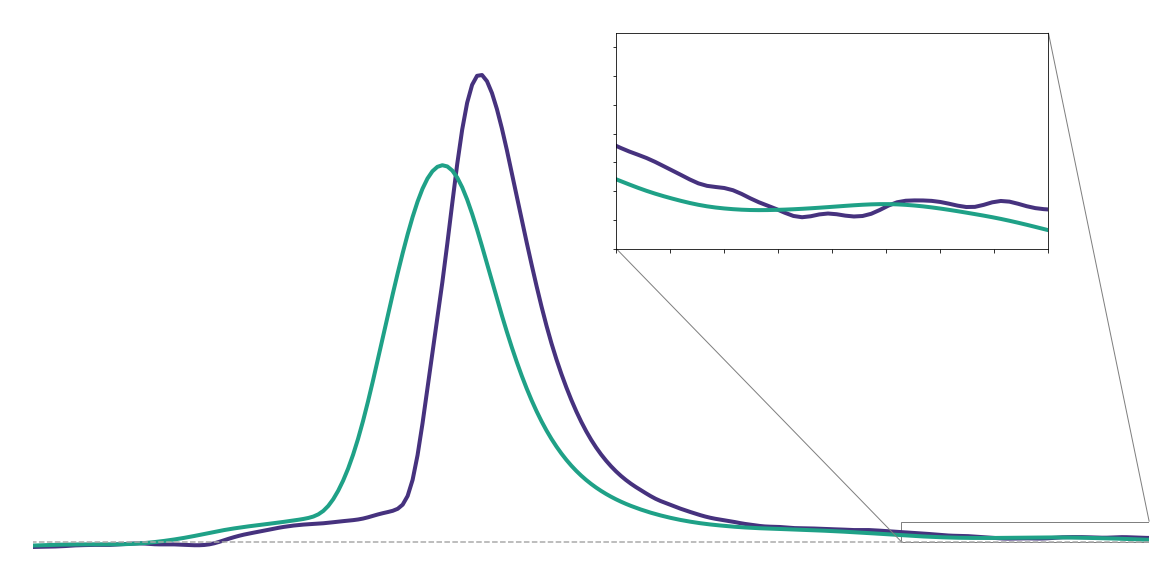
\includegraphics[scale=0.31]{figura1.png} 
%\caption{Simulated time series with AWGN (a) and AWGN + impulsive noise (b). Extracted from \cite{cheffena2016propagation}}
\label{fig:impulsive}
\end{figure*}
\begin{figure*}[h!]
\centering
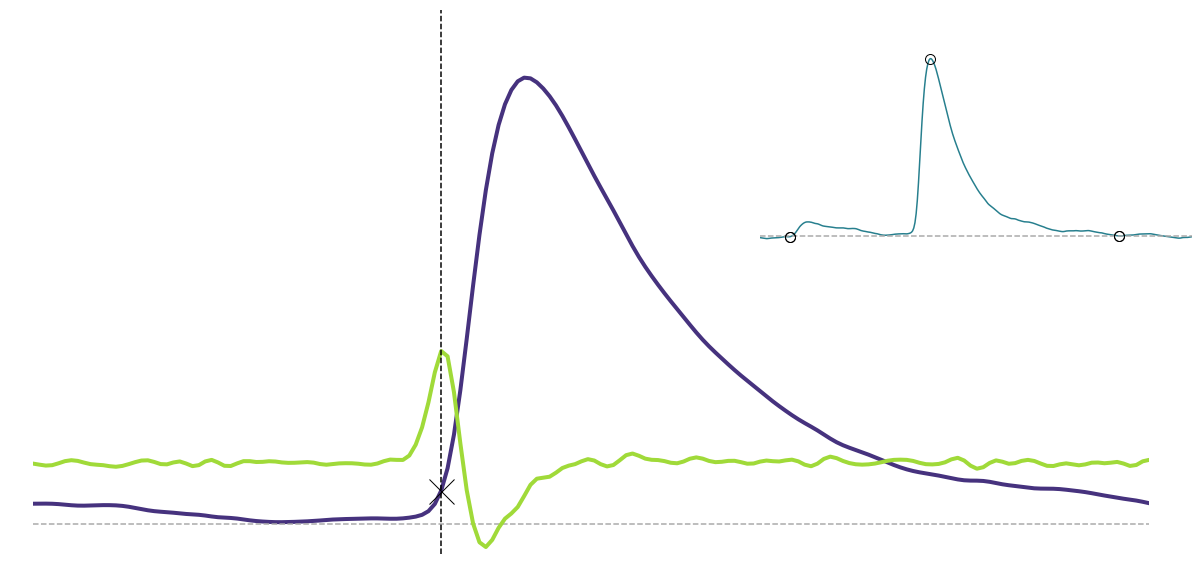
\includegraphics[scale=0.31]{figura2.png} 
\caption{Simulated time series with AWGN (a) and AWGN + impulsive noise (b). Extracted from \cite{cheffena2016propagation}}
\label{fig:impulsive2}
\end{figure*}



\section{Resultados}
\subsection{Pathloss and fading}
Cheffena defined very well the main sources of interference, noise and fading for an Industrial Wireless Channel (IWC).  In particular, in his study\cite{cheffena2016propagation, cheffena2012industrial}, he propose that one of the characteristics for an IWC is the heavy multipath propagation.  Additionaly, he states that no clear relationship between path-loss exponent and frequency can be established for many industrial environment \cite{cheffena2016propagation}.
\subsection{Noise}
Usually, the noise in a wireless communication systems is characterized as AWG.  However, in harsh factory environments, wireless systems are also affected by impulsive noise\cite{low2005wireless,cheffena2016propagation, blackard1993measurements}.
The figure \ref{fig:impulsive} shows this behaviour.  It can be seen that this kind of noise is a significant variable in the performance of a wireless system. 

\subsection{Interference}
As it was stated before, several wireless technologies shares the 2.4GHz ISM band.  In particular, for interference mitigation, IEEE 802.15.4 uses direct sequence spread spectrum (DSSS), dynamic channel selection (DCS), acknowledged transmission and retries (ATR) and clear channel assesment (CCA), to mitigate, avoid interference from other 2.4GHz radio products\cite{cheffena2016propagation}.  Additionally, the channels in this standar are designed so they do not collide with Wi-fi channels.
In \cite{low2005wireless} are shown several narrow and broadband sources that may interfere the wireless channel.
\subsection{Time Varying channel}
The time-varying effects in industrial facilities are mainly caused by movements of workers, robots, trucks or other objects, that may cause time-varying channel conditions\cite{cheffena2016propagation}.
\section{Discusión}
It has been stated that there are several problems regarding the transmission of information from one node to another, in a WSN. In general, the authors agree that there are two methods for establish RF channels\cite{luo2011rf}: Simulation-based methods and measurement-based methods.
Each method has its own advantages and drawbacks.  While a simulation-based method could be cheaper, its computational cost is, sometimes, a burden that must be avoided.  On the other hand, while measurement-based methods are easier to develop, their monetary cost could jeopardize a small research.
The best choice is often, a mix between measure and models. However, the measurement results from one environment may not be applicable to other environment\cite{cheffena2016propagation}.
This big issue lead to several models that try, to the best of their efforts, to achieve certain degree of plausibility, while keeping the computational cost at some affordable quantity. 
\subsection{Industrial Environment}
While most of the researchers try to gather data from the industrial environment and then adjust the data to some existing models\cite{luo2011rf,grote2009wireless}, others develop mathematical models that aim to be as broad and flexible as possible.
Cheffena developed the {\bf Composite Dynamic Wideband Channel Model}\cite{cheffena2012industrial}, in which he models the time varying channel with the combined effect of noise, interferences and multipath propagation. 
In particular, he considers the noise as a mix of AWGN and impulse noise; interference as the sum of the n-arriving signals, considering its power and phase; multipath propagation as result of reflection within an ellipse where the foci are the transmiting and receiving node; and finnaly, a time variation represented by a Doppler spectrum.
The model is then described as followed:


\subsection{Minning Environment}
\begin{figure*}[h!]
\centering
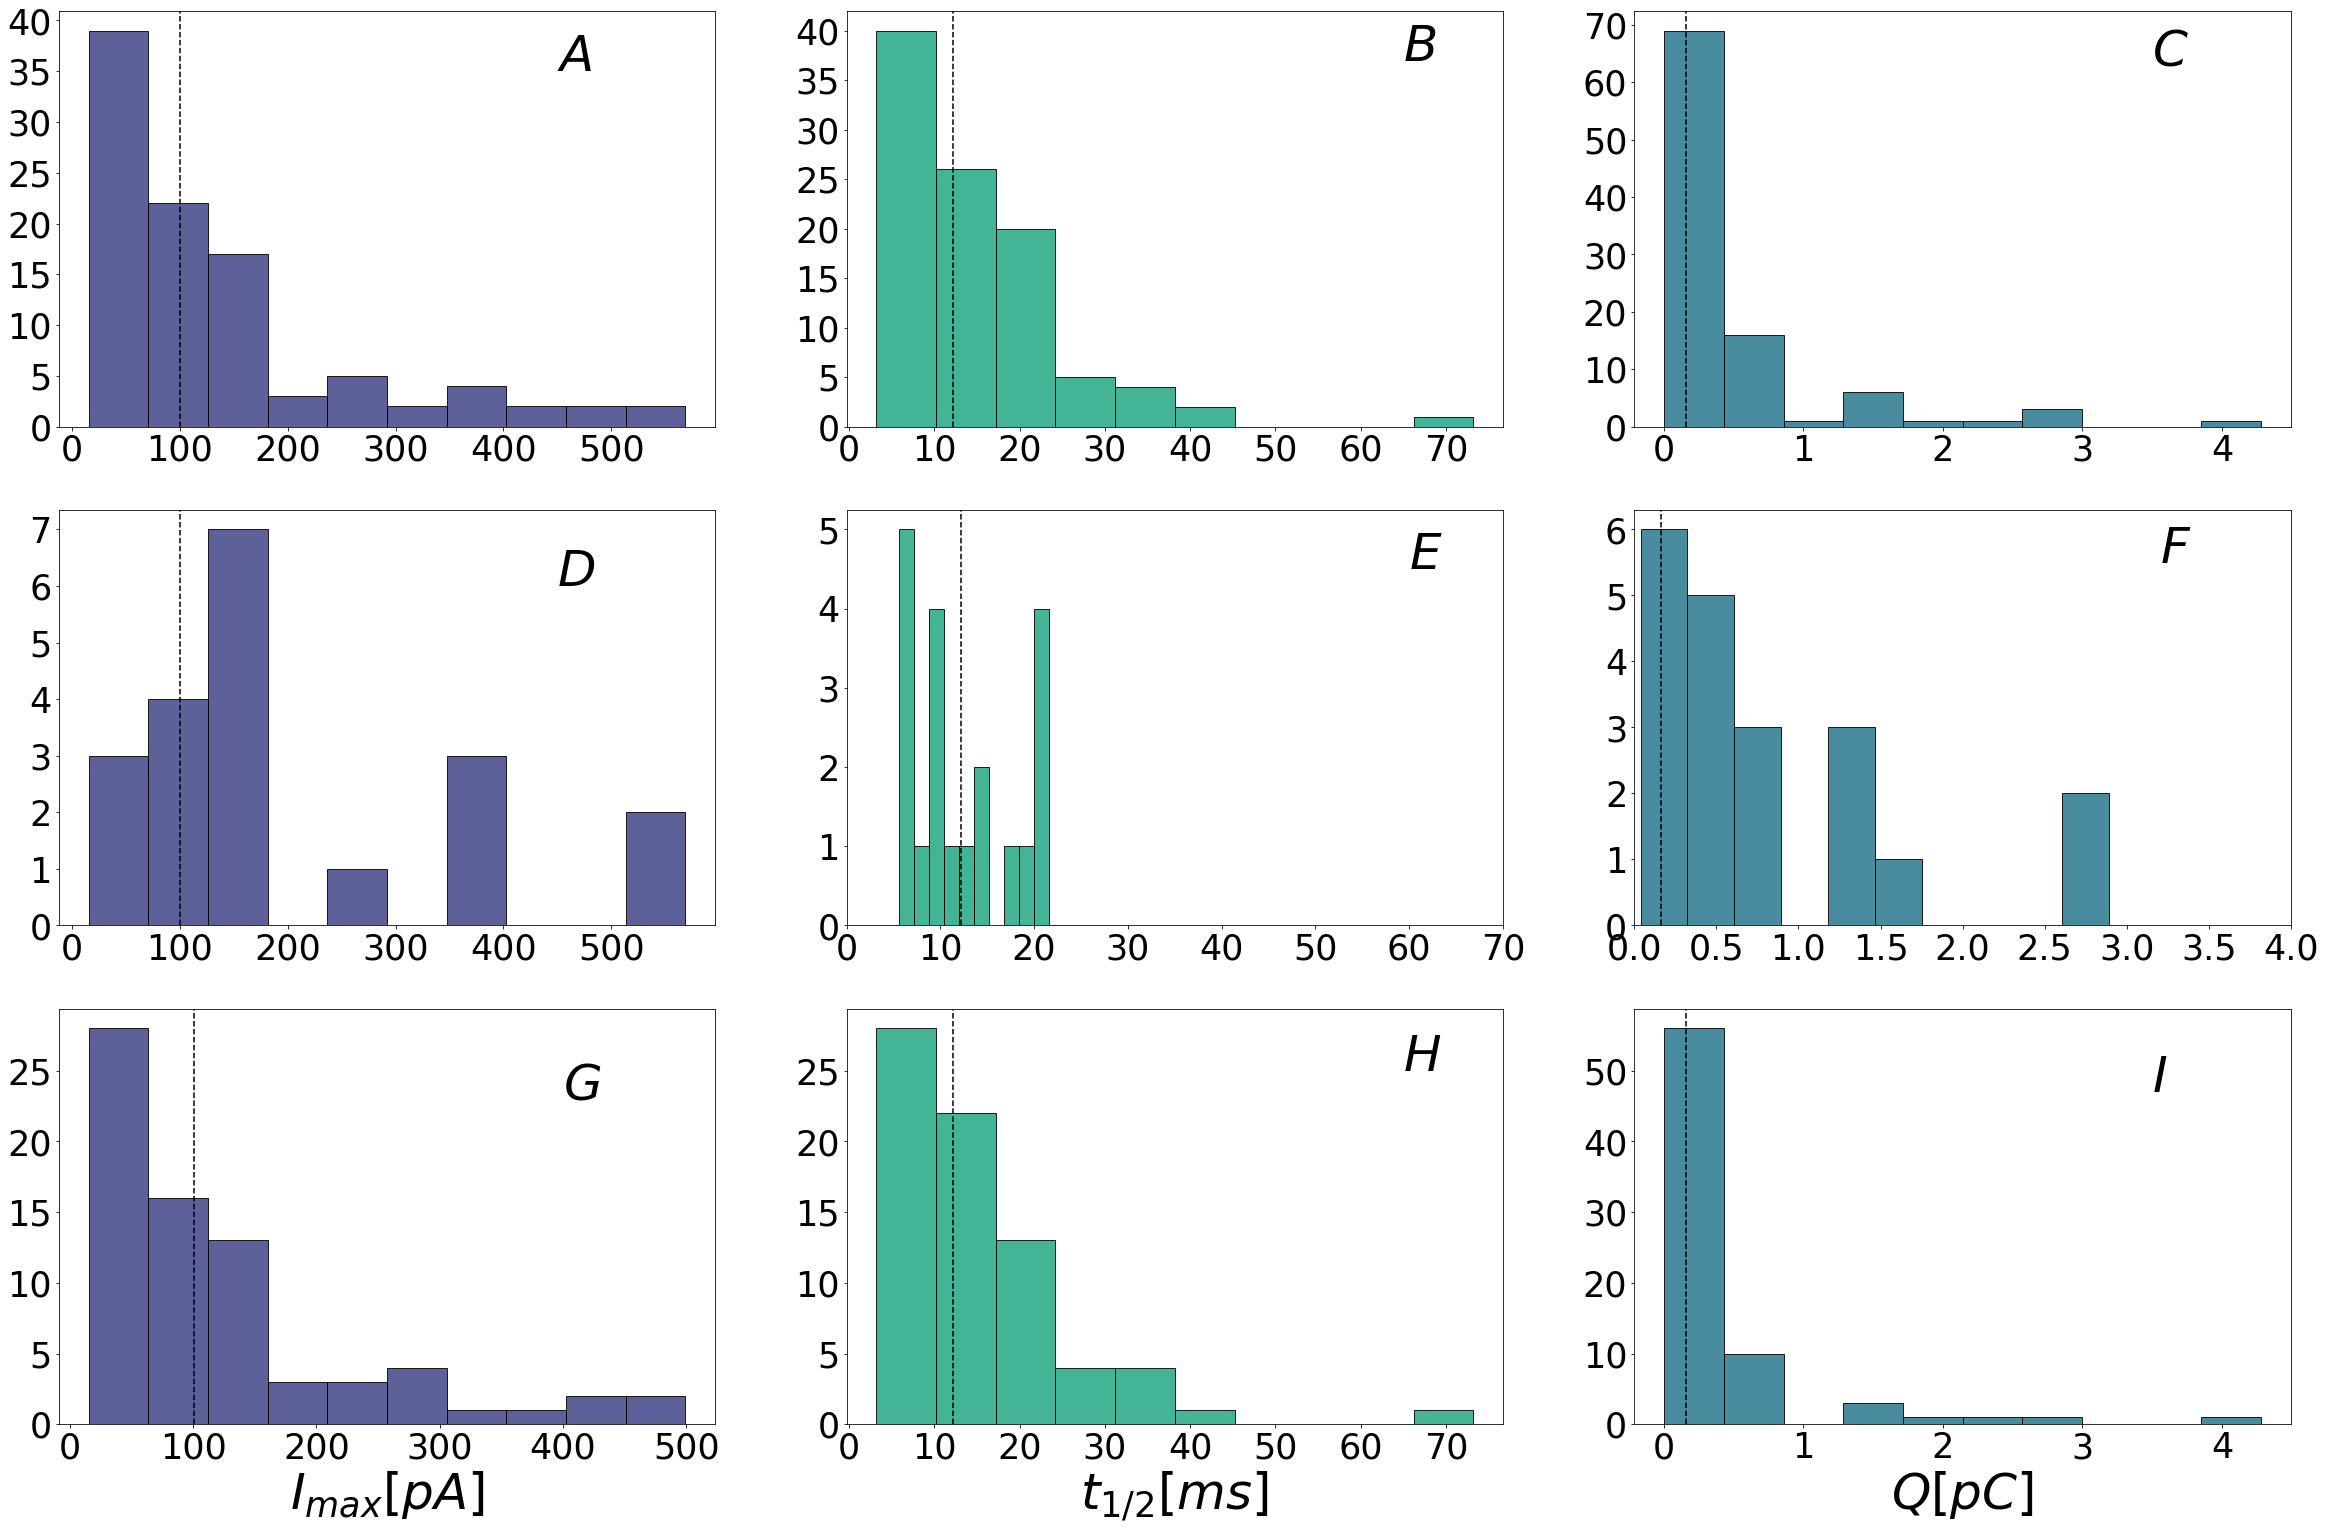
\includegraphics[scale=0.23]{barras.png} 
\caption{Left shows the simulations and experimental data for the multimode model in a Tunnel condition.  The simulation curves are intentionally 75dB below, for comparision purposes.  Right shows the simulation and experimental data in room-and-pilar condition.  Simulated curves are 40dB below for comparision. Extracted from \cite{sun2010channel}}
\label{fig:multimode}
\end{figure*}



On the other hand, Farjow et at. developed a model that divides the mine into three main segments, Line-Of-Sight (LOS), Partial-Line-Of-Sight(PLOS) and Non-Line-Of-Sight(NLOS). This model, called {\bf Mine Segmening Wireless Channel Model}\cite{farjow2015novel}, in contrast with the Multimode model, does not uses Maxwell's equations for developing the model, but instead, uses a combination of statistical models that act together, to characterize a general area or areas within a mine.
\section{Conclusiones}

\clearpage
\newpage

\bibliographystyle{abbrv}
\bibliography{bibliografia}

\end{document}
